
\paragraph{UC-1 Login web}
\begin{itemize}
	\item \textbf{Attore primario:} utente non autenticato; 

	\item \textbf{Descrizione:} l'utente vuole autenticarsi come amministratore presso l'applicazione web. L'operazione di login avrà successo solamente nel caso in cui le credenziali inserite siano corrette ed appartengano ad un amministratore. In caso positivo verrà visualizzata la dashboard relativa;

	\item \textbf{Precondizioni:} l'utente è registrato presso il sistema;

	\item \textbf{Postcondizioni:} l'utente è autenticato ed autorizzato come amministratore presso il sistema;

	\item \textbf{Scenario principale:}
	      \begin{enumerate}
		      \item l'utente avvia l'applicazione web;
		      \item l'utente inserisce le proprie credenziali di accesso ed invia i dati al sistema (UC-1.1 Inserimento credenziali);
		      \item se le credenziali sono corrette, il sistema aggiorna la schermata del dispositivo con la \glo{dashboard} dell'amministratore.
	      \end{enumerate}
\end{itemize}

\begin{figure}[H]
    \centering
      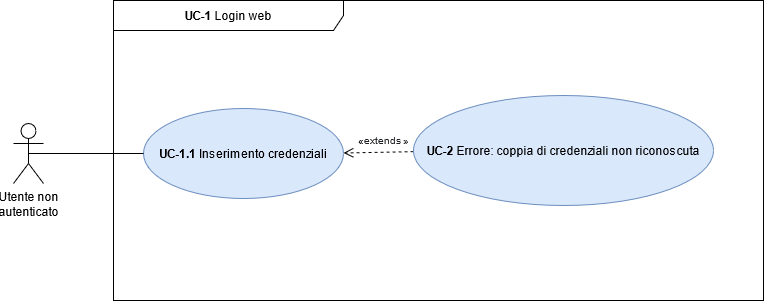
\includegraphics[scale=0.50]{src/CasiDUso/immagini/LoginWeb.png}
    \caption{Diagramma relativo all'autenticazione presso l'applicazione web}
\end{figure}


  \paragraph{UC-1.1 Inserimento credenziali}
  \begin{itemize}
    \item \textbf{Attore primario:} utente non autenticato;
  
    \item \textbf{Descrizione:} l'utente vuole inserire le proprie credenziali (mail e password) per autenticarsi presso l'applicazione web;
  
    \item \textbf{Precondizioni:} l'utente è registrato presso il sistema ed ha avviato l'applicazione web;
  
    \item \textbf{Postcondizioni:} l'utente ha inserito correttamente e-mail e password;
  
    \item \textbf{Scenario principale:}
          \begin{enumerate}
            \item l'utente inserisce il proprio indirizzo e-mail (UC-1.1.1 Inserimento dell'indirizzo e-mail per il login);
            \item l'utente inserisce la propria password (UC-1.1.2 Inserimento della password per il login);
            \item l'utente conferma l'inserimento;
            \item il sistema elabora i dati ed in caso di credenziali errate restituisce un messaggio d'errore esplicativo (UC-2 Errore: coppia di credenziali non riconosciuta), altrimenti procede con la richiesta.
          \end{enumerate}
    \item \textbf{Estensioni:}
      \begin{itemize}
            \item UC-2 Errore: coppia di credenziali non riconosciuta.
          \end{itemize}
  \end{itemize}
  
\begin{figure}[H]
    \centering
      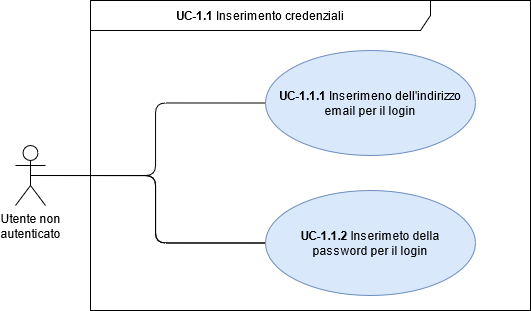
\includegraphics[scale=0.50]{src/CasiDUso/immagini/InserimentoCredenzialiWeb.png}
    \caption{Diagramma relativo all'inserimento delle credenziali nell'applicazione web}
\end{figure}
  
  \paragraph{UC-1.1.1 Inserimento dell'indirizzo e-mail per il login}

	\begin{itemize}
		\item \textbf{Attore primario:} utente non autenticato;

		\item \textbf{Descrizione:} l'utente vuole inserire il proprio indirizzo e-mail nell'apposito form nella schermata di login;

		\item \textbf{Precondizioni:} l'utente ha selezionato il form per l'inserimento dell'indirizzo e-mail;

		\item \textbf{Postcondizioni:} l'utente ha inserito con successo il proprio indirizzo e-mail;

		\item \textbf{Scenario principale:}
	  		\begin{enumerate}
		  		\item l'utente inserisce il proprio indirizzo e-mail nell'apposito form nella schermata di login; 
	  		\end{enumerate}
	\end{itemize}

\paragraph{UC-1.1.2 Inserimento della password per il login}

	\begin{itemize}
		\item \textbf{Attore primario:} utente non autenticato;

		\item \textbf{Descrizione:} l'utente vuole inserire la propria password nell'apposito form nella schermata di login;

		\item \textbf{Precondizioni:} l'utente ha selezionato il form per l'inserimento della password;

		\item \textbf{Postcondizioni:} l'utente ha inserito con successo la propria password;

		\item \textbf{Scenario principale:}
	  		\begin{enumerate}
			  \item l'utente inserisce la propria password nell'apposito form nella schermata di login; 
	  		\end{enumerate}
	\end{itemize}


\paragraph{UC-2 Errore: coppia di credenziali non riconosciuta}
\begin{itemize}
	\item \textbf{Attore primario:} utente non autenticato;

	\item \textbf{Descrizione:} l'applicazione web riconosce solamente le credenziali appartenenti ad un amministratore; l'utente ha provato ad effettuare il login da applicazione web ma ha inserito una coppia di credenziali non valida;

	\item \textbf{Precondizioni:} l'utente ha inserito un indirizzo e-mail e una password errati (o non appartenenti ad un amministratore) ed ha inviato i dati inseriti;

	\item \textbf{Postcondizioni:} il sistema restituisce un messaggio d'errore esplicativo e non completa la richiesta di autenticazione dell'utente;

	\item \textbf{Scenario principale:}
	      \begin{enumerate}
		      \item il sistema non riconosce le credenziali inserite;
		      \item il sistema restituisce un messaggio d'errore esplicativo che viene visualizzato sullo schermo del dispositivo dell'utente e non completa la richiesta di autenticazione.
	      \end{enumerate}
\end{itemize}

\paragraph{UC-3 Logout web}
\begin{itemize}
	\item \textbf{Attore primario:} amministratore;

	\item \textbf{Descrizione:} l'amministratore vuole effettuare il logout dal sistema;

	\item \textbf{Precondizioni:} l'amministratore è autenticato presso il sistema;

	\item \textbf{Postcondizioni:} l'amministratore non è più autenticato presso il sistema;

	\item \textbf{Scenario principale:}
	      \begin{enumerate}
		      \item l'amministratore seleziona la funzionalità di logout;
		      \item il sistema elabora la richiesta e aggiorna la schermata riportandola a quella d'avvio dell'applicazione e rendendo indisponibile l'accesso alla dashboard dell'amministratore fino a nuovo accesso.
	      \end{enumerate}
\end{itemize}


